\subsection{Mixed Reality und HoloLens}
\label{sec-2-1}

\subsubsection{Mixed Reality}
\label{sec-2-1-1}
\fbox{
	\parbox{\linewidth}{
		\textit{Ziel des Kapitels:}\\
		Begriffsklärung und Einordnung von AR,MR,VR in das Virtual Continuum. Wichtig für die Einordnung von MR in Education in \ref{sec-2-2}.\\[6px]
		\textit{Inhalte:}	
		\begin{itemize}
			\item Virtual Continuum erklären und AR, AV, VR einordnen
		\end{itemize}
		
		\textit{Wichtige Literatur:}	
		\begin{itemize}
			\item A taxonomy of mixed reality visual displays \cite{Milgram94}
			\item A survey of augmented reality \cite{Azuma97}
			\item Augmented Reality: Where we will all live \cite{Peddie17}
		\end{itemize}
}}

\begin{figure}[h!]
	\centering
	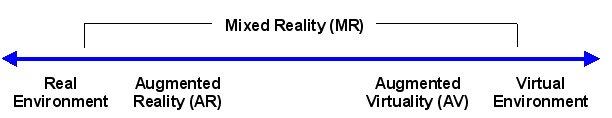
\includegraphics[width=0.9\textwidth]{images/virtual_continuum.png}
	\caption{Virtual Continuum eingeführt von Paul Milgram \cite{Milgram94}}
	\label{img:virtual_continuum}
\end{figure}

kurz andere Techniken erwähnen, damit unterschiedliche Arbeiten entsprechend eingeordnet werden können. Smartphone AR, z.B. Apple ARKit, Pokemon Go, HUDs, Oculus Rift, Vive, PS VR, Opaque vs see through, standalone vs wired, Bezug zu anderen Techniken ansprechen: Object detection, Object recognition, Object tracking

HoloMuse, Galaxy Explorer, Fragments, LifeLiqe, HoloTour, Insight Heart, Dynamic Anatomy\\
Damit Orientierungshilfe gegeben und Vorstellungsvermögen verbessert für späteres Anwendungsdesign

Leistungssteigerung im Hardwarebereich und Fortschritte bei AI führt zur Verfügbarkeit von Devices von AR bis VR, daher sehr aktuelles Thema, viel Potential

\subsubsection{HoloLens}
\label{sec-2-1-2}
\fbox{
\parbox{\linewidth}{
	\textit{Ziel des Kapitels:}\\
	HoloLens und Mixed Reality Toolkit mit ihrer Technik und Interaktionsweise vorstellen (und auf Implikationen für das Design eingehen.)\\[6px]
	\textit{Inhalte:}	
	\begin{itemize}
		\item Übersicht über Technik der HoloLens, besonderer Fokus auf Designrelevanten Aspekten
		\item Interaktion und MRTK (kurz) vorstellen
		\item Kurz ansprechen, dass die Technik Auswirkungen auf das Design hat
	\end{itemize}

	\textit{Wichtige Literatur:}	
	\begin{itemize}
		\item Mobile Augmented Reality Illustrations That Entertain and Inform: Design and Implementation Issues with the Hololens \cite{Zimmer17}
		\item Microsofts eigene Docs
		\item Ggf. Resourcen zu technischen Quellen bezüglich eingesetzter Techniken
	\end{itemize}
}}
	

HMD mit see through display, 60hz upscale zu 240hz, jede Farbe einzeln sequenziell, pro Anwendungsframe also 3 Farbframes, inside out tracking mit IMU, 2x IR und Stereo Kamera, Head Movement Prediction, Standalone, CPU, GPU, Akkulaufzeit, Gewicht, Windows 10 Holographic, Entwicklung und Deployment mit Unity

\textbf{Interaktion}\\

Gestensteuerung, Click, Hold-Click, Drag-Drop, Scale, Bloom usw. 1 und 2 Hand Gesten, Anwendungen können per API auf Gesten reagieren, Sprachsteuerung (Englisch), API für Spracherkennung\\

\textbf{Implikationen für Anwendungsdesign}

Abstand, Geschwindigkeit und Größe der Objekte wichtig, Blickwinkel, Depth Cues, Drop Shadows, Occlusion, Einführung in Gesten, FoV, Cursor, Weiß - Rainbow, Dunkle Farben vermeiden, Performance, Klick-Feedback